% Essential Formatting

\documentclass[12pt]{article}
\usepackage{epsfig,amsmath,amsthm,amssymb}
\usepackage[questions, answersheet]{urmathtest}[2001/05/12]
%\usepackage[answersheet]{urmathtest}[2001/05/12]
%\usepackage[answers]{urmathtest}[2001/05/12]


% For use with pdflatex
% \pdfpagewidth\paperwidth
% \pdfpageheight\paperheight

% Basic User Defs

\def\ds{\displaystyle}

\newcommand{\ansbox}[1]
{\work{
  \pos\hfill \framebox[#1][l]{ANSWER:\rule[-.3in]{0in}{.7in}}
}{}}

\newcommand{\ansrectangle}
{\work{
  \pos\hfill \framebox[6in][l]{ANSWER:\rule[-.3in]{0in}{.7in}}
}{}}


% Beginning of the Document

\begin{document}
\examtitle{LINEAR REGRESSION MODELS W4315}{HOMEWORK 3}{09/16/2009}
 \begin{center}
  Instructor: Frank Wood\\
 You are not allowed to use build-in regression functions in matlab. Pdf and cdf of common distributions are allowed. Attach relevant and concise code to your homework. Hand in a hard copy.
 \end{center}
%%\studentinfo
\instructions{
  %\textbf{Circle your Instructor's Name along with the Lecture Time:}



  \begin{itemize}
  \item
    \textbf{Please show all your work.
            You may use back pages if necessary.}
  %\item
   % \textbf{Please put your \underline{simplified}
   %         final answers in the spaces provided.}
  \end{itemize}
}
\finishfirstpage

% Problems Start Here % ----------------------------------------------------- %


\problem{25} {\footnote[1]{This is
problem 2.5 in ``Applied Linear Regression Models(4th edition)'' by
Kutner etc.}
 Refer to \textbf{Copier maintenance} homework 1 problem 4. Find the data in ``copier.txt''.\\
 a. Estimate the change in the mean service time when the number of copiers serviced increases by one. Use a 90 percent confidence interval. Interpret your confidence interval.\\
 b. Conduct a \textit{t} test to determine whether or not there is a linear association between X and Y here; control the $\alpha$ risk at .10. State the alternatives, decision rule, and conclusion. What is the p-value of your test?\\
 c. Are your results in parts (a) and (b) consistent? Explain.\\
 d. The manufacturer has suggested that the mean required time should not increase by more than 14 minutes for each additional copier that is serviced on a service call. Conduct a test to decide whether this standard is being satisfied by Tri-City. Control the risk of a Type I error at .05. State the alternatives, decision rule, and conclusion. What is the p-value of the test?\\
 e. Does $b_0$ give any relevant information here about the ``start-up'' time on calls-i.e., about the time required before service work is begun on the copiers at a customer location?
   }
 { \vfill
  \answer
} {
a. $t(.95; 43) = 1.6811$, $15.0352 \pm 1.6811(.4831)$, $14.2231 \leq \beta_1 \leq 15.8473$\\
b. $H_0: \beta_1 = 0$, $H_a: ��\beta_1 \neq 0$. $t^* = (15.0352 - 0)/.4831 = 31.122$. If $|t^*| \leq 1.681$
conclude $H_0$, otherwise $H_a$. Conclude $H_a$. P-value = 0+\\
c. Yes\\
d. $H_0: \beta_1 \leq 14$, $H_a: \beta_1 > 14$. $t^* = (15.0352 - 14)/.4831 = 2.1428$. If $t^* \leq 1.681$
conclude $H_0$, otherwise $H_a$. Conclude $H_a$. P-value = .0189\\
e. No, it doesn't make practical sense and thus provides no relevant information.
}

\problem{25} {\footnote[2]{This is
problem 2.13 in ``Applied Linear Regression Models(4th edition)'' by
Kutner etc.}
The director of admissions of a small college selected 120 students at
random from the new freshman class in a study to determine whether a student's grade
point average(GPA) at the end of the freshman year($Y$) can be predicted from the ACT
test score($X$). You can find the data in the file ``GPA.txt'', the first column is $Y$ and the
second is $X$. Assume a simple linear regression model with normal error terms.\\
a. Obtain a 95 percent interval estimate of the mean freshman GPA for students whose ACT
test score is 28. Interpret your confidence interval.\\
b. Mary Jones obtained a score of 28 on the entrance test. Predict her freshman GPA using a 95 percent prediction interval. Interpret your prediction interval.\\
c. Is the prediction interval in part (b) wider than the confidence interval in part (a)? Should
it be?\\
d. Determine the boundary values of the 95 percent confidence band for the regression line
when $X_h = 28$. Is your confidence band wider at this point than the confidence interval in
part (a)? Should it be?
   }
 { \vfill
  \answer
} {
a. $\hat{Y}_h = 89.6313$, $s\{\hat{Y}_h\} = 1.3964$, $t(.95; 43) = 1.6811$, $89.6313 \pm 1.6811(1.3964)$,
$87.2838 \leq E\{Y_h\} \leq 91.9788$\\
b. $s\{pred\} = 9.0222$, $89.6313 \pm 1.6811(9.0222)$, $74.4641 \leq Y_{h(new)} \leq 104.7985$, yes,
yes\\
c. $87.2838/6 = 14.5473$, $91.9788/6 = 15.3298$, $14.5473 \leq Mean time per machine
\leq 15.3298$\\
d. $W^2 = 2F(.90; 2, 43) = 2(2.4304) = 4.8608$, $W = 2.2047$, $89.6313 \pm 2.2047(1.3964)$,
$86.5527 \leq \beta_0 + \beta_1X_h \leq 92.7099$, yes, yes
}

\problem{25} {\footnote[1]{This is
problem 3.4 in ``Applied Linear Regression Models(4th edition)'' by
Kutner etc.}
 Refer to \textbf{Copier maintenance}.\\
 a. Prepare a dot plot for the number of copiers serviced $X_i$. What information is provided by this plot? Are there any outlying cases with respect to this variable?\\
 b. The cases are given in time order. Prepare a time plot for the number of copiers serviced. What does your plot show?\\
 d. Prepare residual plots of $e_i$ versus $\hat{Y_i}$ and $e_i$ versus $X_i$ on separate graphs. Do these plots provide the same information? What departures from regression model (2.1) can be studied from these plots? State your findings. And the model (2.1) is as follows:
 \[Y_i=\beta_0+\beta_1 X_i+\epsilon_i\]
 where:\\
 $\beta_0$ and $\beta_1$ are parameters\\
 $X_i$ are known constants\\
 $\epsilon_i$ are independent $N(0,\sigma^2)$\\

 e. Prepare a normal probability plot of the residuals. Also obtain the coefficient of correlation between the ordered residuals and their expected values under normality(use the approximation given in (3.6) of textbook). Does the normality assumption appear to be tenable here? Use Table B.6 of the textbook and set $\alpha=.10$.\\
 h. The file ``copier\_more.txt'' provides two more variables into consideration(the third and fourth column), namely, mean operational age of copiers serviced on the call($X_2$, in months) and years of experience of the service person making the call($X_3$). Plot the residuals against $X_2$ and $X_3$ on separate graphs to ascertain whether the model can be improved by including either or both of these variables. What do you conclude?\\
N.B. \textbf{You don't need to do part c, f and g.}
}
 { \vfill
  \answer
} { 
a. No obvious outlying cases.
	\begin{center}
	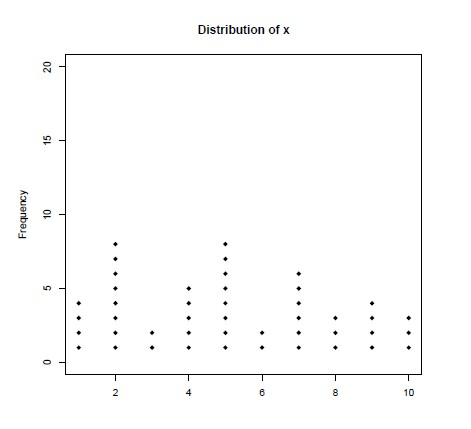
\includegraphics[width=.7\textwidth]{1.jpg}
	\end{center}
b. No particular trend.
\begin{center}
	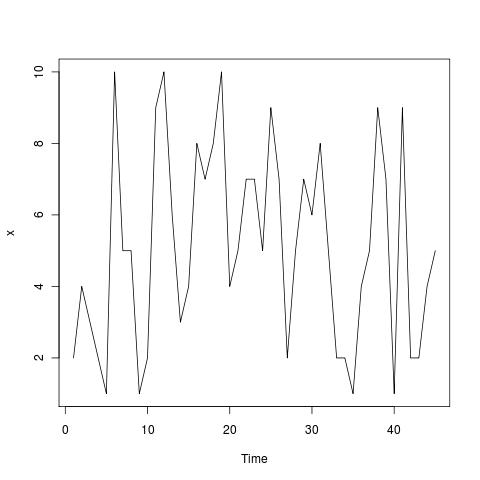
\includegraphics[width=.7\textwidth]{2.jpg}
	\end{center}
\begin{center}
	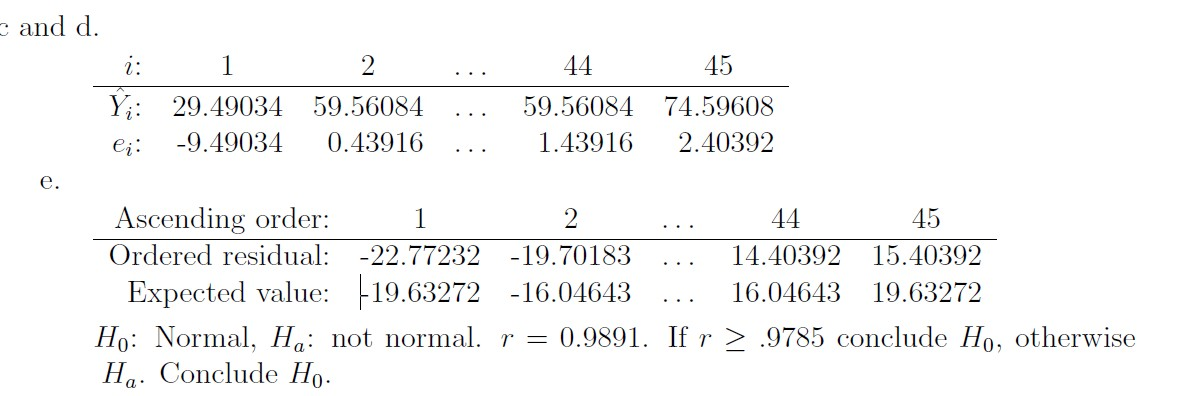
\includegraphics[width=\textwidth]{34de.jpg}
	\end{center}

h. From the graph below, we can see that adding $X_2$ might improve the model (a strong linear
relations between residuals and $X_2$), while adding $X_3$ seems to be not that useful.
\clearpage
\begin{figure}[!h]
\begin{center}
	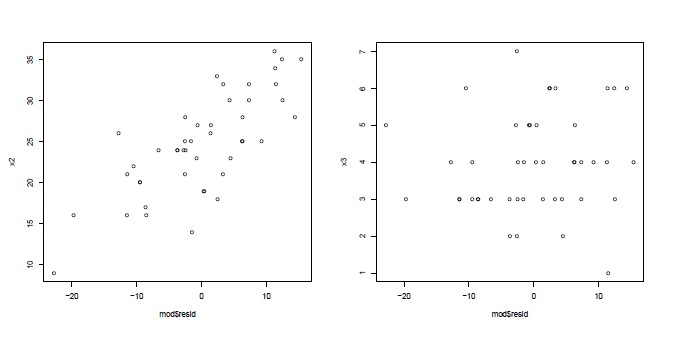
\includegraphics[width=\textwidth]{3.jpg}
\centerline{\bf Left is for X2, right is for X3.}
	\end{center}
\end{figure}
}

\problem{25} {
 In normal probability plot (also referred to as Q-Q plot), we draw the expectation
of the order statistics from normal distribution against the observed ordered residuals. If
the error terms are indeed normal, then we should expect to see a linear relationship. Now
consider a simplified situation, $X_1, X_2, X_{3},\ldots,X_{10} \text{ i.i.d.} \sim N(0,1)$.\\
 a. Write out the probability density functions of order statistics $X_{(1)}, X_{(5)} $ and $ X_{(10)}$. ($X_{(i)}$ is
the $i$th largest item in $X_1, X_2, X_{3},\ldots,X_{10} $.)\\
 b. Draw the pdf of $X_{(1)},X_{(5)} $ and $X_{(10)}$ on one graph.\\
 c. What are the expected values of $X_{(1)},X_{(5)} $ and $X_{(10)}$?(Use the approximation given in (3.6) of textbook).
Mark them on the graph.
}
 { \vfill
  \answer
} {
a. The pdf of order statistics $X_{(k)}$ is
$$f_{X_{(k)}}(x)= \frac{n!}{(k-1)!(n-k)!}F(x)^{k-1}(1-F(x))^{n-k}f(x)$$
in which $F(x)$ is the cdf of standard normal and $f(x)$ is the pdf of standard normal. n = 10.\\
b. The graph is given below
\begin{center}
	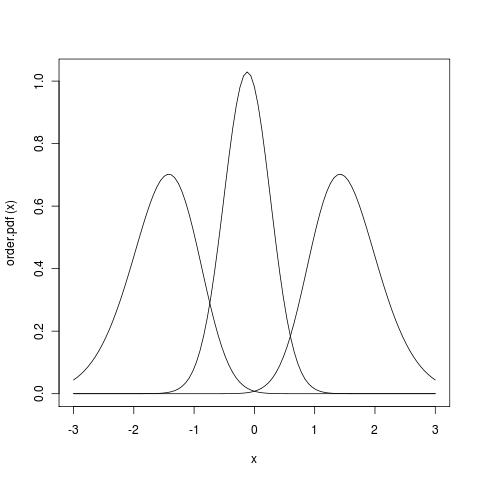
\includegraphics[width=.7\textwidth]{4.jpg}
	\end{center}
c. Expectations are $EX_{(1)} = -1.55$,$EX_{(5)} = -0.122$, $EX_{(10)} = 1.55$
}



% Problems End Here % ------------------------------------------------------- %

\problemsdone
\end{document}

% End of the Document
